\section{Natural forecasting: transfer, cost, and predicting benefit}\label{sec:natural}

\subsection{A separate source-level evaluation}
The natural study fixes four development families (Electricity, NN5,
Tourism, and FRED-MD) and four confirmation families (Traffic, Hospital,
Saugeen River flow, and US births). Versions, licenses, eligibility rules,
and chronological windows are specified in Appendix~\ref{sec:nf-protocol}.
Training-prefix eligibility and a fixed salted ordering select 26 series.
Two history--horizon regimes, two capacities, and two seeds yield 208 runs:
128 development and 80 confirmation. Related series, windows, horizons,
capacities, and seeds remain within their original source families.
The units describing transfer breadth are the four confirmation families.

Each series uses chronological 60/20/20 percent training/validation/test
blocks, and every target horizon lies entirely within its split. All
learned transformations and feature bases use the permitted training
data. Validation chooses hyperparameters; a final refit uses eligible
pretest targets, and test outcomes never retune parameters. Contexts can
use earlier observed values. At most 64 validation and 64 test origins
are retained by a fixed spacing rule; missing windows are excluded
identically for every method, without interpolation or replacement series.
Mean-squared forecast error is divided by a fixed initial-training
seasonal-difference scale. Aggregation gives each source family equal
weight, followed by its nested task levels. These descriptive quantities
are not pooled with the controlled-study confidence families.

The twelve candidates include raw ridge and raw finite-RBF predictors;
affine-, locality-, and KAHM-gated local predictors, with and without the
full raw history; and seasonal naive, Holt, histogram boosting, and a small
MLP. The primary matched pair is raw RBF ($R$) versus raw plus KAHM ($K$).
The raw-augmented code is
\begin{equation}\label{eq:natural-raw}
 T_{\mathrm{raw}+g}(x)=\bigl(z(x),\,\phi_g(z(x)),\,
       (\phi_{g,c}(z(x))P_c^\top(z(x)-\mu_c))_c\bigr).
\end{equation}
It retains every standardized history coordinate. For a fixed fitted state
the raw input is therefore recoverable and Bayes information is unchanged
(Proposition~\ref{prop:nf-raw-preservation}). Finite fitted performance
can still change: appended features alter Gaussian distances, the
Nystr\"om basis, and ridge regularization, and the resulting nonlinear
classes need not be nested.

Small/medium configurations cap training windows at 512/1,024 and RBF
landmarks at 32/64. Each method fits its own preprocessing and geometry;
affine/locality alternatives never fit a KAHM kernel. Within a method,
features and head statistics are reused across penalties $\{0.01,1,100\}$.
The selected model is refitted from scratch. These are specified finite
procedures, not equally timed or exhaustively tuned algorithms. Detailed
heads, practical controls, capacity caps, and numerical conventions appear
in Appendices~\ref{sec:nf-methods}--\ref{sec:nf-protocol}.

\subsection{Which computational work is charged?}
Measured warm-library pipelines include required preparation/loading,
preprocessing, validation search, selection bookkeeping, chosen refitting,
forecasting, and serialization. Libraries are initialized beforehand;
imports and process launch are separately exposed. Wall and CPU time,
model bytes, and process high-water memory have distinct recorded scopes.
Let $S_m$ denote method $m$'s search nodes, $F_m$ its final fit and forecast,
and $m^*$ a validation-selected candidate. Its charged work is
\begin{equation}\label{eq:main-cost}
 C_{\rm val}=\sum_{v\in\mathcal D_{\rm data}\cup
             (\bigcup_{m\in\mathcal A}S_m)\cup F_{m^*}}c_v
             +c_{\rm decision}.
\end{equation}
Unique dependency nodes are counted once. A diagnostic selector likewise
pays for all required descriptors and probes, even when it rejects KAHM.
Acquiring development labels and fitting the small diagnostic regressions
are separate offline investments. No assumed deployment count is used to
amortize them. The costs describe measured implementations on one CPU
environment; they are not intrinsic complexity or hardware-independent
speed ratios.

\subsection{Accuracy and cost on reserved sources}
All 208 declared runs completed with every candidate present; saved
forecasts reconstruct all 2,496 task--method losses. Table~\ref{tab:natural-main}
retains all twelve confirmation candidates. Raw plus KAHM has
\NaturalErrorIncrease\% higher aggregate error than raw RBF, at
\NaturalCostRatio{} times its measured warm-library pipeline cost. Raw
ridge has lower aggregate error than both. Against raw RBF, KAHM raises
mean loss by 0.50\% on Traffic, 12.27\% on Hospital, and 3.53\% on US births;
it lowers loss by 1.53\% on Saugeen, where raw ridge also performs better.
Leaving out any one confirmation family still leaves the KAHM aggregate
above raw RBF. This sensitivity check is descriptive and does not turn
four selected sources into a population-wide inference.

\begin{table}[t]
\centering\small
\caption{All twelve standalone methods on the reserved natural sources. Scaled MSE and warm-library wall time use equal source-family weights and the frozen within-source hierarchy. Times include required preprocessing, search, refitting, prediction, serialization, and measured bookkeeping; imports and launch are separate. These are descriptive results from four source families.}
\label{tab:natural-main}
\begin{tabular}{lrr}
\toprule
Method & Scaled MSE & Wall seconds per task \\
\midrule
Raw ridge & 0.7798 & 0.1880 \\
Raw RBF & 0.8075 & 0.1688 \\
Affine local & 0.9449 & 0.5002 \\
Locality local & 0.8964 & 0.2898 \\
KAHM local & 0.9354 & 0.3218 \\
Raw + affine & 0.8458 & 0.3379 \\
Raw + locality & 0.8462 & 0.2791 \\
Raw + KAHM & 0.8419 & 0.3874 \\
Seasonal naive & 1.0498 & 0.1614 \\
Holt & 2.3729 & 0.3449 \\
Histogram boosting & 0.9555 & 8.9103 \\
MLP & 0.8785 & 1.4626 \\
\bottomrule
\end{tabular}
\end{table}


The structural controls clarify attribution. Raw plus KAHM improves
aggregate loss over raw plus affine and raw plus locality by only 0.46\%
and 0.50\%, respectively. Each comparison favors KAHM on two source
means and the control on two; KAHM costs 14.65\% and 38.82\% more.
These mixed differences do not identify nonlinear reconstruction as a
general source of advantage. At the small/medium settings, KAHM raises
loss against raw RBF by about 2.00/6.70\%; the settings change both
sample caps and model sizes, so their effects are not separately identified.

The favorable development mean also needs qualification. KAHM reduced
loss against raw RBF by 42.45\%, but FRED-MD supplied 96.62\% of the
net absolute reduction. Removing that family reduces the apparent gain
to 4.65\%. Raw plus affine had lower mean loss and cost than KAHM in
each development family, and raw ridge had the lowest overall development
loss. Consequently, the development comparison alone did not establish
a KAHM-specific benefit.

Implementation overhead is substantial. Selection cleanup, including
explicit garbage collection, contributes 0.1381 of raw RBF's 0.1688 seconds
and 0.1825 of KAHM's 0.3874 seconds. Search and final refit are also
reported separately (Table~\ref{tab:cleanup-costs}). The 2.30-fold ratio
describes the supplied warm workflow; it is not a cold-start end-to-end
deployment ratio. Figure~\ref{fig:accuracy-cost} retains the full accuracy--cost
comparison, including selectors that must pay to choose a model.

\begin{figure}[t]
\centering
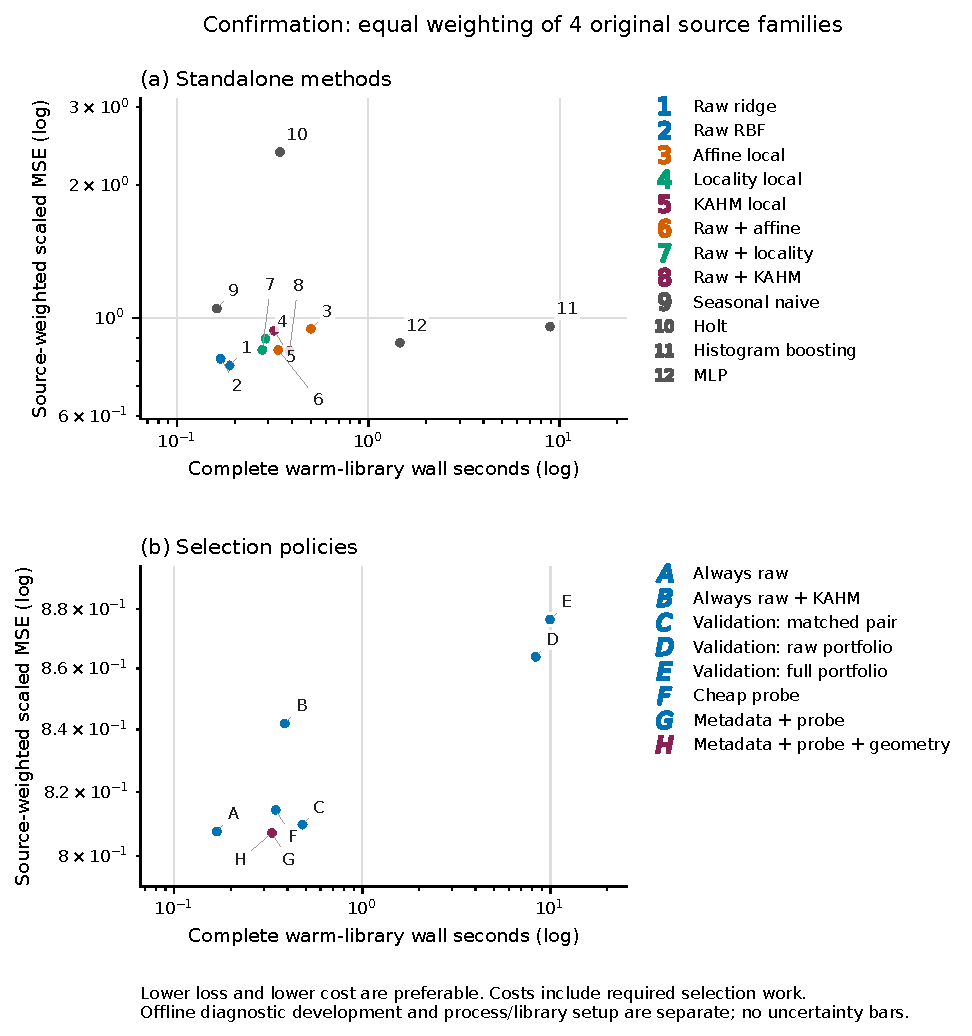
\includegraphics[width=\linewidth]{generated/natural/figures/accuracy_cost.pdf}
\caption{Reserved-source accuracy and measured warm-library cost. All points
use the same source hierarchy. The standalone and selector panels have
separate scales so that all declared candidates remain visible. Selector
costs include required searches and probes. Confirmation outcomes are used
to evaluate these procedures, not to fit a new selection rule.}
\label{fig:accuracy-cost}
\end{figure}

\subsection{The frozen benefit diagnostic}
Four fixed ridge diagnostics predict
$\log[(\ell_R+10^{-12})/(\ell_K+10^{-12})]$ from metadata $M$,
$M$ plus geometry $G$, $M$ plus a cheap validation probe $P$, or $M+P+G$.
Metadata describe training size, horizon/history ratio, and lag-one
autocorrelation; geometry adds gate entropy and an affine-projection
residual. The paid probe compares reduced-capacity raw/KAHM fits on
validation data. A positive estimated log benefit selects KAHM; ties
select raw. Development standardization and training hold out whole source
families. All variants are then fitted on development and frozen before
confirmation; confirmation outcomes cannot choose the variant or threshold.

The primary geometric increment, $M+P+G$ versus $M+P$, changes none of
the 80 confirmation decisions. Both achieve scaled MSE
\NaturalProbeLoss{} at about \NaturalProbeCost{} seconds. The probe already
computes the geometric descriptors, so they need no extra bank fit in this
pair. Log-benefit RMSE nonetheless increases from 0.184549 to 0.184680.
The shared decision rule improves aggregate loss over always raw by only
\NaturalProbeGainPercent\%, at \NaturalProbeCostRatio{} times its pipeline
cost. It improves one source mean, worsens one, and ties two.
Metadata-plus-geometry also makes exactly the same choices as metadata
alone, while paying for extra feature acquisition. All variants and
validation-portfolio controls remain in Table~\ref{tab:policy-summary}.

Offline learning requires more than fitting a small ridge regression.
Acquiring the matched development outcomes and shared probe/metadata
dependencies costs 80.83 seconds of summed measured pipeline work;
all four final ridge fits together add about 0.032 seconds. Shared
dependencies must not be added repeatedly across variants. These
observations provide no validated geometric adoption criterion for the
tested procedure. They also do not establish that usefulness is
unpredictable by a different, independently evaluated diagnostic.
